\begin{frame}\frametitle{\vspace*{0.5cm}I aim to further our understanding of the relevant fluid mechanics}
  \begin{figure}
    \centering%
    \hfill%
    \begin{tikzpicture}%
      \node[anchor=south west,inner sep=0] (image) at (0,0) {%
        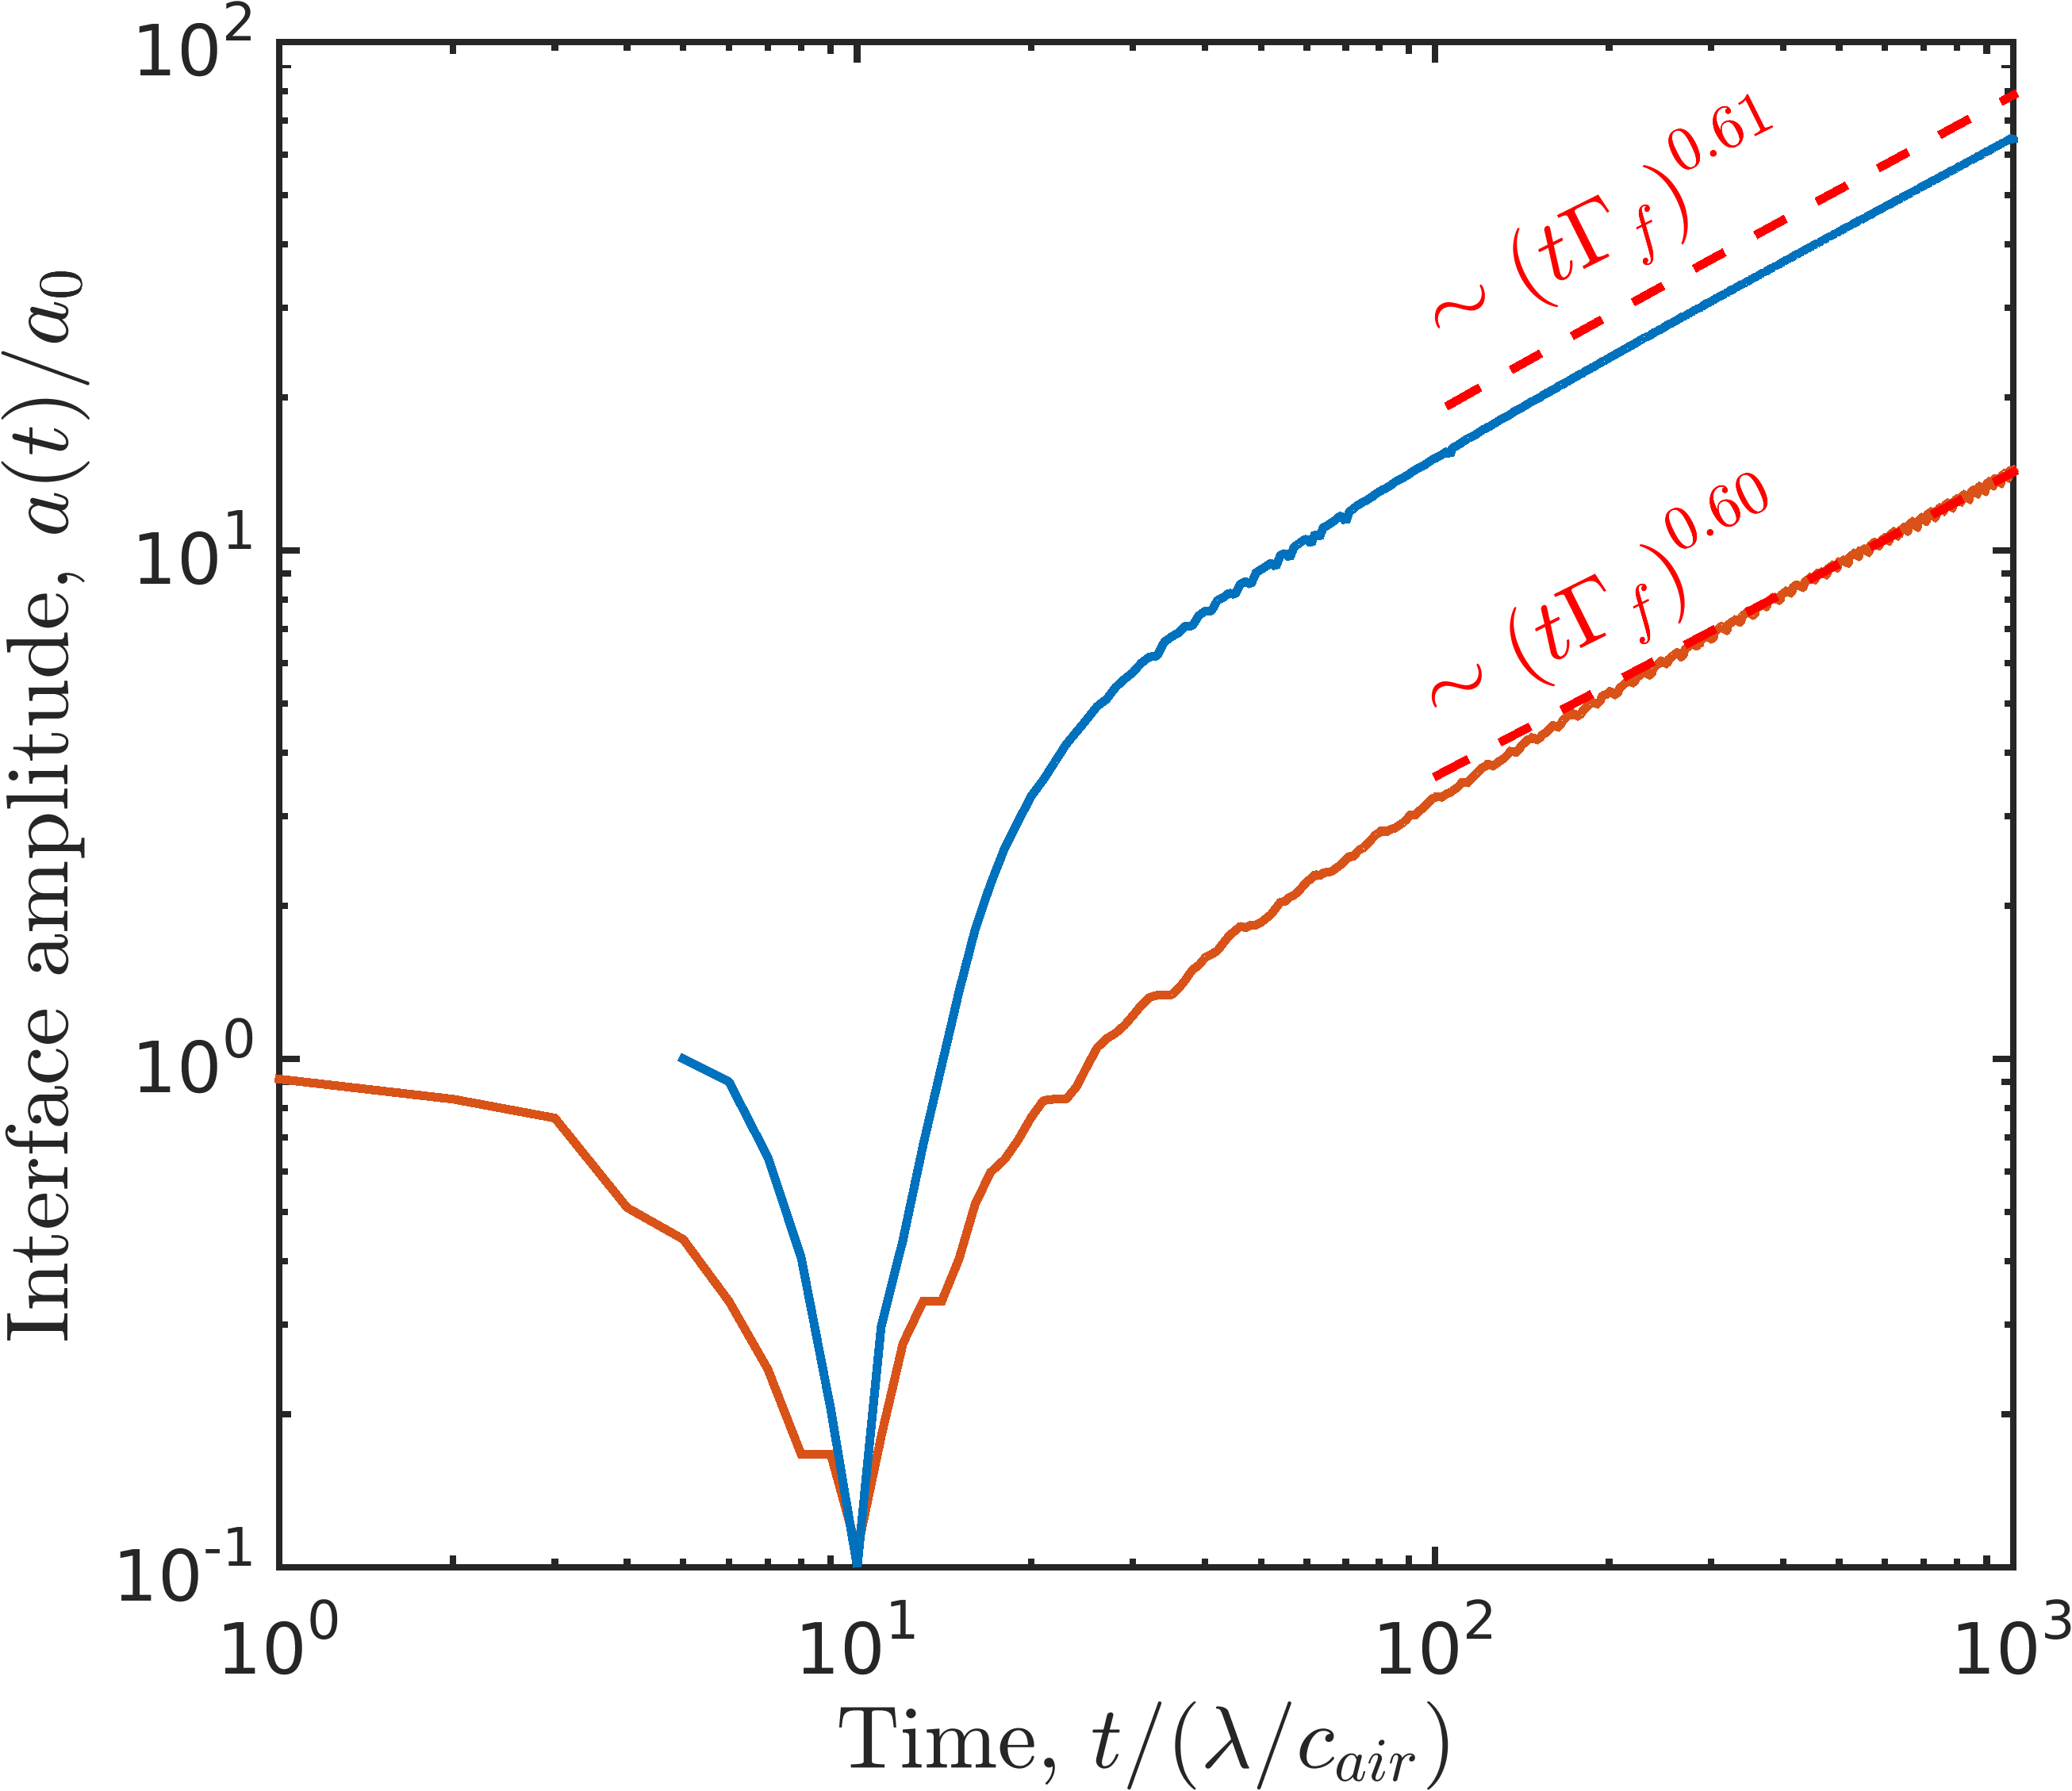
\includegraphics[height=0.45\textheight]{../figs/lung_figs/interface_multi-amp_loglog_roe_t1000}%
      };%
      \begin{scope}[x={(image.south east)},y={(image.north west)}]%
        \node[font=\footnotesize,right] at (0.32,0.7){ $10$ MPa};%
        \node[font=\footnotesize,right] at (0.55,0.4){ $5$ MPa};%
      \end{scope}%  
    \end{tikzpicture}%
    \hfill%
    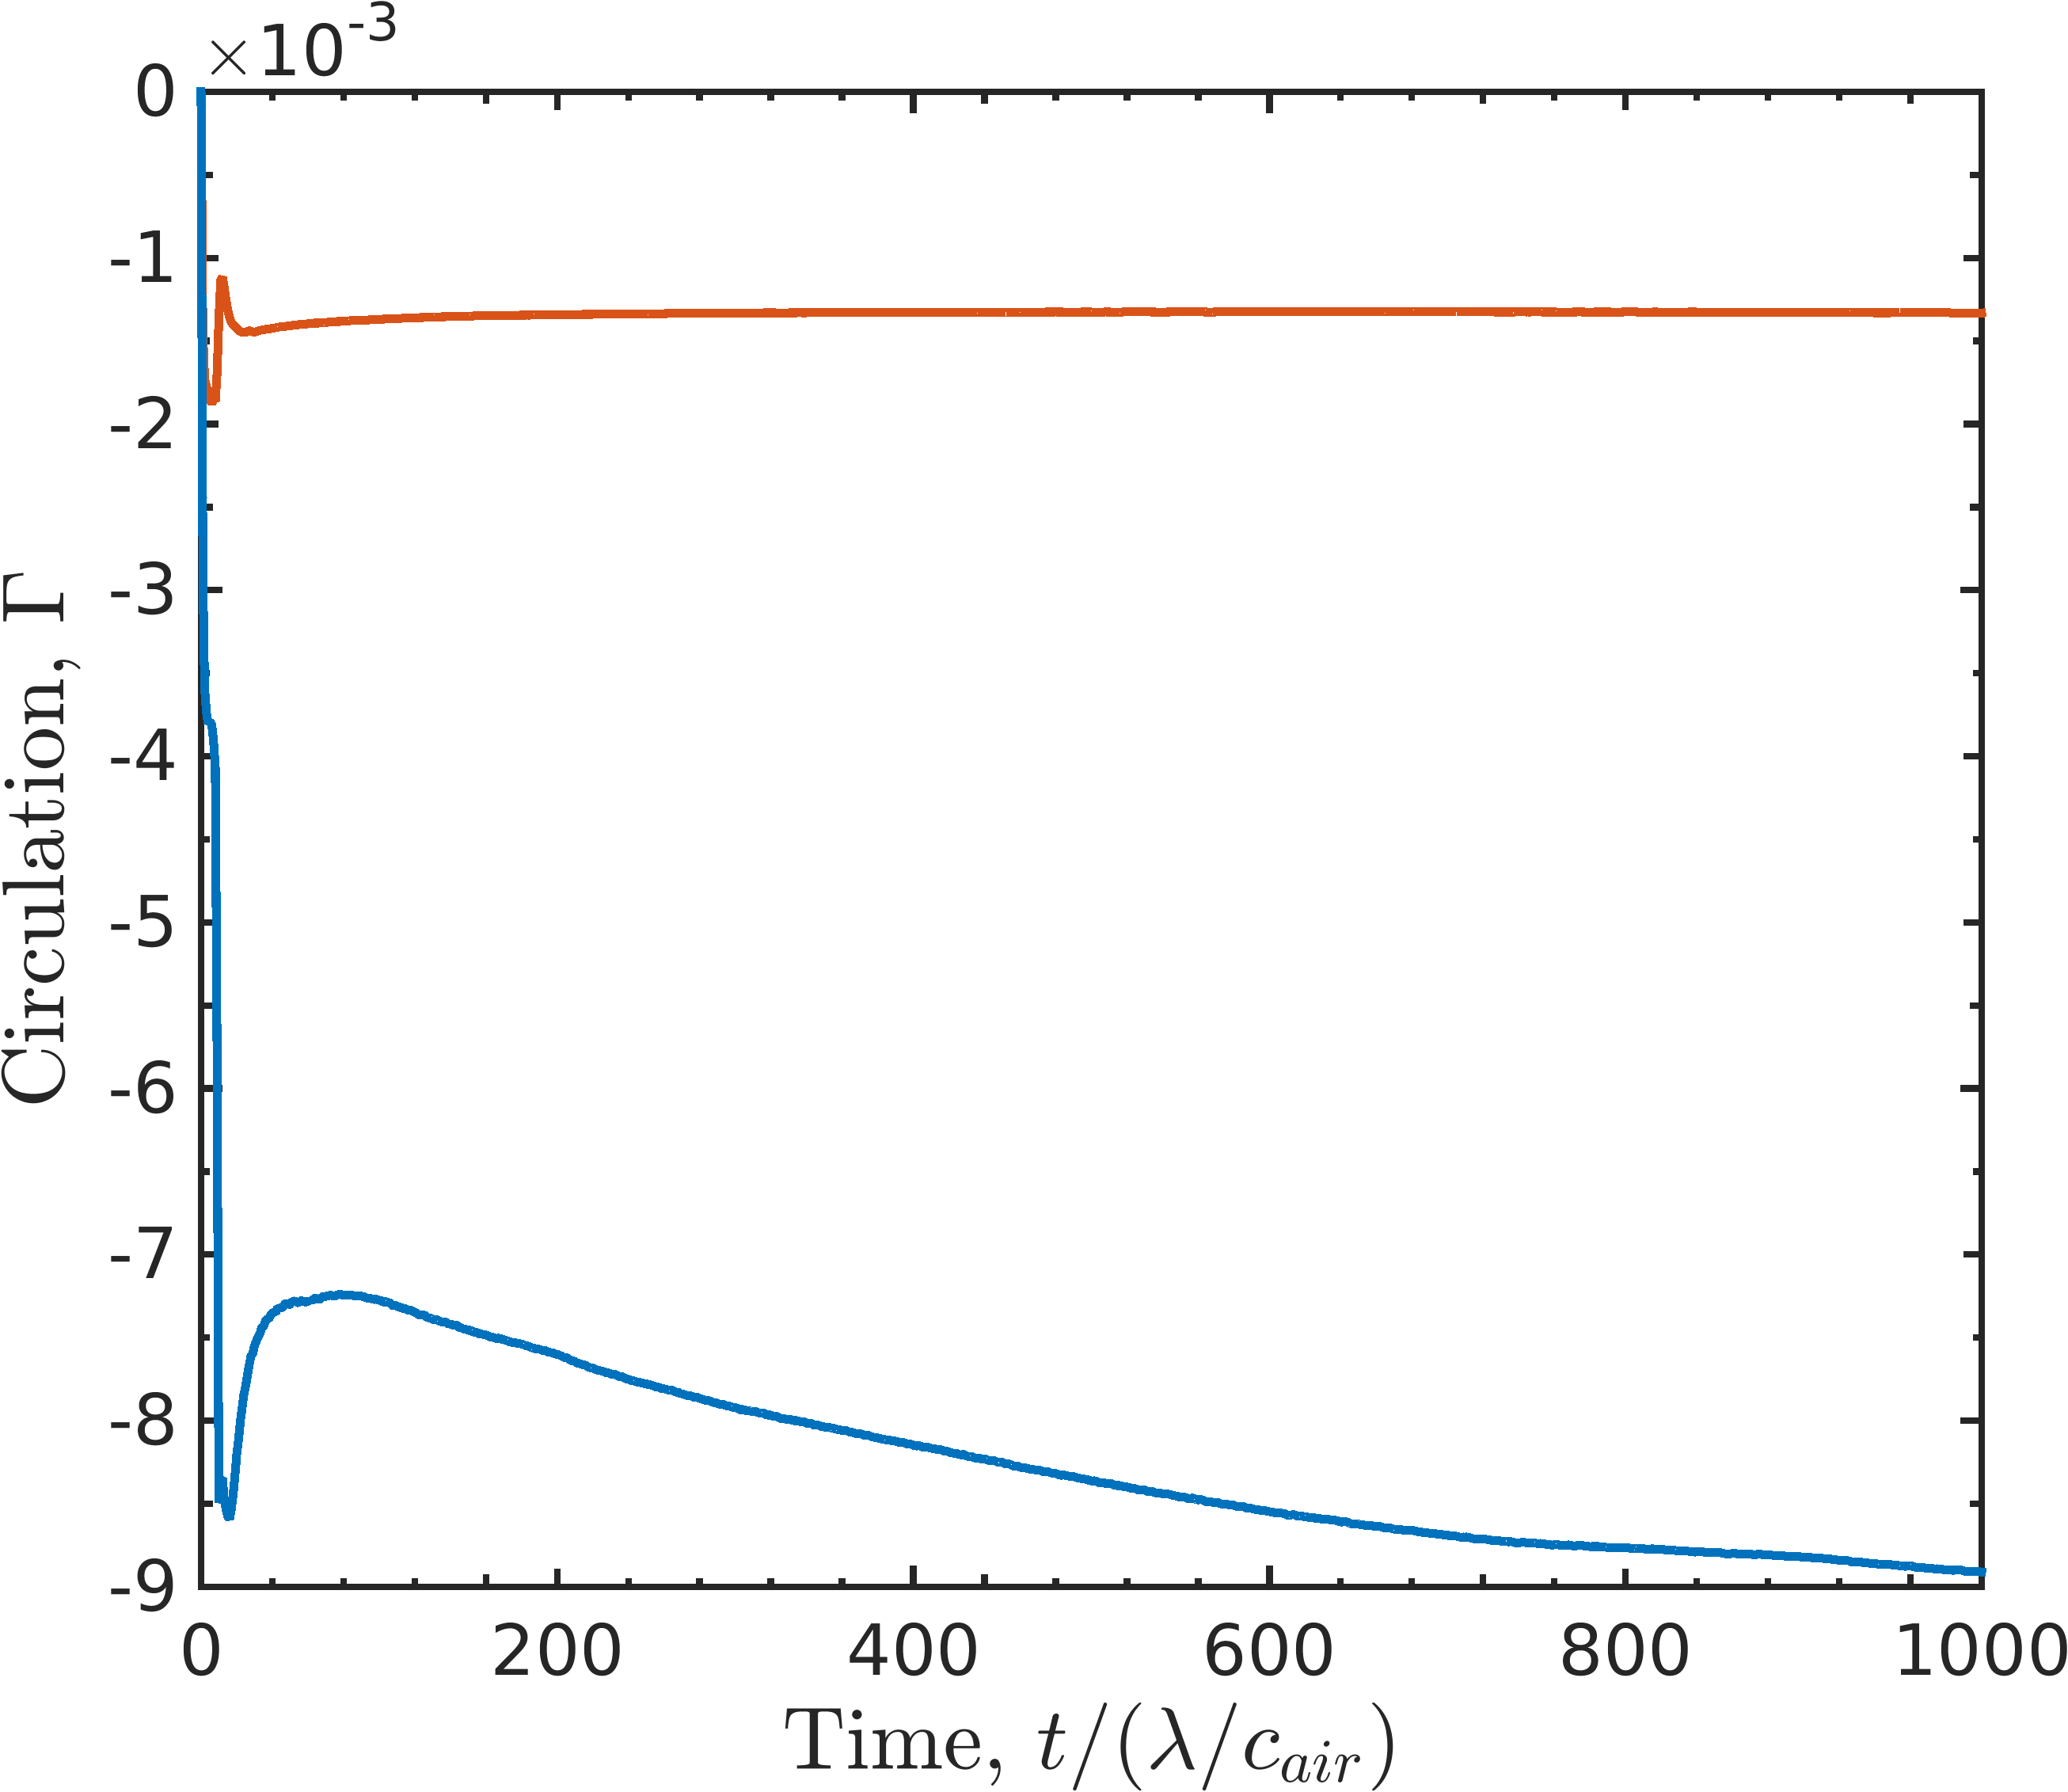
\includegraphics[height=0.45\textheight]{../figs/lung_figs/circulation_multi-amp_roe_t1000}%
    \hfill%
  \end{figure}
  % 
  {\small
    \begin{itemize}
    \item Explain the discrepancies between numerical results and $a(t)\sim\sqrt{\Gamma t}$%
      \vspace*{5pt}
    \item Develop a model and scaling law $\Gamma(\nabla p, a_0)$ to for circulation deposited on a
      slightly perturbed interface by a compression or expansion wave
      \vspace*{5pt}
      % \item Develop a model to predict the interface phase-reversal time for a compression wave
      %   \vspace*{5pt}
%    \item Design an acoustic waveform to minimize circulation and interface growth.
%      \vspace*{5pt}
    \item Invert the waves to confirm counter rotating vertices relevant growth
    \end{itemize}
  }
\end{frame}
%
%%% Local Variables:
%%% mode: latex
%%% TeX-master: "../main"
%%% End:
